%% ACM article template
%\documentclass[sigconf,authordraft]{acmart}         % Draft, one column.
%\documentclass[sigconf, anonymous, review]{acmart}  % Draft, anonymous.
\documentclass[sigconf, nonacm]{acmart}              % arXiv version.
%\documentclass[sigconf]{acmart}                      % Final version.

%\documentclass[manuscript,screen]{acmart}           % One column.
%\documentclass[manuscript]{acmart}
%\documentclass{article}

%\newcommand{\Description}[1]{}
%\usepackage{booktabs}
%\usepackage{graphicx}
%\usepackage{comment}
%\usepackage{longtable}

%% \BibTeX command to typeset BibTeX logo in the docs
\AtBeginDocument{%
  \providecommand\BibTeX{{%
    \normalfont B\kern-0.5em{\scshape i\kern-0.25em b}\kern-0.8em\TeX}}}

%\begin{comment}
%% These commands are for a PROCEEDINGS abstract or paper.
\acmConference[BeyondFacts'24]{4th International Workshop on Computational Methods for Online Discourse Analysis}{May 13--17, 2024}{Singapore}

%% ACM stuff:
%% Rights management information.
\setcopyright{acmcopyright}
\copyrightyear{2024}
\acmYear{2024}
\acmDOI{XXXXXXX.XXXXXXX}
% Price:
%\acmPrice{15.00}
\acmPrice{00.00}
\acmISBN{978-1-4503-9419-2/24/05}
%% Submission ID.
%%\acmSubmissionID{123-A56-BU3}
%\end{comment}

\begin{document}
\title{Identifying groups of interest in W3C}

%% Authors:
\author{Henrique S. Xavier}
%\authornote{Both authors contributed equally to this research.}
%\begin{comment}
\email{hxavier@nic.br}
\orcid{0000-0002-9601-601X}
%\authornotemark[1]
\affiliation{%
  \institution{NIC.br}
  \streetaddress{Av. das Nações Unidas, 11541, 7º andar}
  \city{São Paulo}
  \state{SP}
  \country{Brazil}
  \postcode{04578-000}
}
\author{Beatriz Rocha}
%\authornote{Both authors contributed equally to this research.}
%\begin{comment}
\email{biarocha@nic.br}
%\orcid{0000-0002-9601-601X}
%\authornotemark[1]
\affiliation{%
  \institution{NIC.br}
  \streetaddress{Av. das Nações Unidas, 11541, 7º andar}
  \city{São Paulo}
  \state{SP}
  \country{Brazil}
  \postcode{04578-000}
}


% Authors for header:
%\renewcommand{\shortauthors}{Xavier et al.}
\renewcommand{\shortauthors}{H. S. Xavier}
%\end{comment}

%% Abstract:
\begin{abstract}

Let's check who participates in the W3C and what are their interests.
  
\end{abstract}

%%
%% The code below is generated by the tool at http://dl.acm.org/ccs.cfm.
%% Please copy and paste the code instead of the example below.
%%
%\begin{comment}
\begin{CCSXML}
<ccs2012>
   <concept>
       <concept_id>10002951.10003260</concept_id>
       <concept_desc>Information systems~World Wide Web</concept_desc>
       <concept_significance>500</concept_significance>
       </concept>
   <concept>
       <concept_id>10003456.10003457.10003490</concept_id>
       <concept_desc>Social and professional topics~Management of computing and information systems</concept_desc>
       <concept_significance>500</concept_significance>
       </concept>
   <concept>
       <concept_id>10010405.10010455</concept_id>
       <concept_desc>Applied computing~Law, social and behavioral sciences</concept_desc>
       <concept_significance>300</concept_significance>
       </concept>
   <concept>
       <concept_id>10003456.10003457.10003567</concept_id>
       <concept_desc>Social and professional topics~Computing and business</concept_desc>
       <concept_significance>300</concept_significance>
       </concept>
 </ccs2012>
\end{CCSXML}

\ccsdesc[500]{Information systems~World Wide Web}
\ccsdesc[500]{Social and professional topics~Management of computing and information systems}
\ccsdesc[300]{Applied computing~Law, social and behavioral sciences}
\ccsdesc[300]{Social and professional topics~Computing and business}
%% Keywords:
\keywords{world wide web, standards, W3C, SDO, topic modelling, web science}

%% A "teaser" image:
%\begin{teaserfigure}
%  \includegraphics[width=\textwidth]{images/dalle_smiley_network_teaser}
%  \caption{A painting expressing the associations between sentiments.}
%  \Description{A painting of smiley faces connected by lines as nodes in a network.}
%  \label{fig:teaser}
%\end{teaserfigure}

\received{19 April 2024}
%\received[revised]{12 March 2009} % arXiv
%\received[accepted]{5 June 2009}  % arXiv
%\end{comment}

\maketitle

\section{Introduction}
\label{sec:intro}

%\subsection{Motivation}
%\label{sec:motivation}

The Web has changed significantly the way we communicate, study, work, and live, and today it is an indispensable element to inumerous human activities. Since its creation in 1989, the Web itself has changed significantly, often in unexpected directions. Initially designed as an academic information system for sharing documents in a descentralized way \cite{BernersLee1990}, the Web gained the capacity to host interoperable, dynamic, interactive, and real-time applications including Software-as-Service (SaaS), e-commerce, social media, and streaming services, while facilitating or allowing for new practices such as monitoring, testing and nudging users \cite{Zuboff2019} and profiting from crowdsourcing, wisdom of the crowds, user-generated content, data mining, and targeted advertising \cite{OReilly2005}. Also, user activity and content got contentrated in a few for-profit platforms \cite{Xavier2024}. 

From the history of the Web, it is clear that foreseeing its development can be extremely valuable both in economic and social terms. Albeit challenging, studying the current state of the Web, its actors and their focus of interest can provide evidence of the Web's possible future directions. Some studies have pursued this path, each using different indicators. \cite{Xavier2024} analyzed online traffic data from SimilarWeb and identified key industries and pervasive practices encountered by users on the Web, along with the main controllers of the most popular websites, whereas \cite{Graux2022} explored the topics covered in the Web Conference series, identifying historical and new trends in Web-related research. These studies confirm the importance of Big Tech US companies in driving research and shaping user experience on the Web, of video streaming services, business models based on crowdsourcing content from users or third parties, and of employing artificial intelligence on the Web, specially as recommender systems. In contrast, once thought as the future of the Web \cite{BernersLee2001}, the Semantic Web was found stalled in research and not much used in practice \cite{Hogan2020}.

Our goal is to complement these studies by analyzing the participation of different actors in the World Wide Web Consortium (W3C), the main standards development organization (SDO) for the Web. The W3C is responsible for many standards and best practices that govern the Web and its members include large and small companies, non-profit organizations, government institutions, and academia. By studying the activity of these actors in W3C, we can gain insights into their interests and priorities, as well as the potential impact of their work on the future of the Web.

%\subsection{Previous research on W3C}
%\label{sec:previous}

The main W3C activities take place in groups\footnote{\url{https://www.w3.org/groups}}. These can be split into permanent groups and temporary groups. There are four permanent groups, which have governance and oversight attributions: the Advisory Board (AB), the Technical Architecture Group (TAG), the Advisory Committee (AC) and the Board of Directors (BoD). The temporary groups are created to work on specific topics related to the Web standards and practices and are expected to disband after their work is done. These groups are divided into chartered and non-chartered groups. Only W3C members can participate in chartered groups, while non-chartered groups are open to anyone. The former groups are further divided into Working Groups (WG) and Interest Groups (IG), while the latter are divided into Community Groups (CG) and Business Groups (BG). Despite WGs being the only one that can produce W3C Recommendations (a.k.a standards)\footnote{\url{https://www.w3.org/standards/types/\#x5-standard}}, all group types are considered relevant for the development of the Web. The community and business groups, for instance, are seen as incubators for new ideas and technologies and may create momentum for a later standarization\footnote{\url{https://www.w3.org/community/about/faq}} \cite{Harcourt2020}.

Previous publications about the W3C have reported that, although counting with members from academia, government, and civil society, large companies are the main players, followed by smaller ones \cite{Gamalielsson2016, Halpin2017, Harcourt2020, Mason2019}. The latter pattern in common in other SDOs. According to \cite{Harcourt2020}, most standards are submitted to the W3C after they have been developed and implemented, typically when the need for interoperability becomes apparent, and ``most salient work within the W3C is led mainly by browser companies such as Google and Microsoft, manufacturers like Intel, and user companies such as Facebook'' while ``Comcast and Netflix are also important actors particularly within specifications for television.'' A 2016 analysis of the filiations of the editors of W3C standards revealed the collaboration between universities and large and small companies and the dominance of organizations based in the United States \cite{Gamalielsson2016}. The latter finding was also highlighted in an analysis of the mailing list of the W3C HTML WG, which also identified negligible participation from Asia, Africa and South America and by women in general \cite{Gupta2016}. Studies specifically focused on the W3C Encrypted Media Extensions (EME) Recommendation delved into mailing lists activity and participation in related groups, identifying similar patterns \cite{Halpin2017, Mason2019}.

Using distinct indicators -- namely, Recommendation editorships, participation in W3C groups, and activity in mailling lists -- the referred works reached an important conclusion about the overall composition of the W3C: the predominance of large companies, especially from the USA and Europe. Presumably, it is the interests of these participants that will guide the evolution of Web standards. However, previous studies did not differentiate the companies (by industry sector, for instance) and did not analyze the topics of interest of these participants. This paper aims to fill this gap by identifying the W3C members' interests, as expressed in the temporary groups they participate in, and use this information to discover latent topics and interest groups in W3C. Besides revealing the topics being driven by strong Web players, our analysis can also detect fields left to other organizations and that can flourish subject to different interests. 

%\subsection{About W3C}
%\label{sec:w3c}
 
\section{Data Set}
\label{sec:data}

The data used in this paper is publicly available on W3C's website and API and allows for the identification of the organization each W3C group participant is affiliated to. For each organization we collected information on whether it is a member of W3C, and for members we were able to collect their headquarters country. We also used retrieval-augmented generation (RAG, described in Sec. \ref{sec:rag}) to annotate the sector of each member organization under the following categories: 
\begin{itemize}
  \item \textbf{Large enterprises}: for-profit companies with more than 250 employees.
  \item \textbf{Small and medium enterprises (SMEs)}: for-profit companies with up to 250 employees.
  \item \textbf{Non-profit organizations}: non-profit organizations, including NGOs and foundations.
  \item \textbf{Government}: government institutions, including intergovernmental organizations. 
  \item \textbf{Academia}: universities and research institutions.
  \item \textbf{Technical communities}: technical communities, including standards development organizations (SDOs) and open source projects.
\end{itemize}
These sectors are mainly based on the multi-stakeholder groups adopted by the Internet Governance Forum (IGF)\footnote{\url{https://www.intgovforum.org/en/about\#about-igf-faqs}} and NET mundial\footnote{\url{https://netmundial.br/2014}}, with an extra breakdown in the private sector inspired by \cite{Gamalielsson2016,Harcourt2020}. A manual check of 60 organizations indicated an accuracy of 87\% for the RAG-annotated sectors.

Table \ref{tab:sources} summarizes the data sources used in this paper, along with our own identification scheme and collection date. Given that the member organization headquarter's countries data were collected several months after the rest of the data, 30 organizations may have left W3C and did not figure in \texttt{country}. Thus, we filled the missing data by manually checking Wikipedia and the organizations' websites. Fig. \ref{fig:data-structure} presents a graph visualization of our data relations.



\begin{table*}[ht]
  \caption{Data sources}
  \label{tab:sources}
  \begin{tabular}{lllr}
    \toprule
    \textbf{Data ID} & \textbf{Description} & \textbf{Source} & \textbf{Collection date} \\
    \midrule
    \texttt{listing} & W3C Groups listing & \url{https://api.w3.org/groups} & 2024-07-25 \\
    \texttt{groups} & Groups properties & \url{https://api.w3.org/groups/{group}} & 2024-07-25 \\
    \texttt{users} & Groups participants & \url{https://api.w3.org/groups/{group}/users} & 2024-07-25 \\
    \texttt{affiliations} & Participants' organization & \url{https://api.w3.org/users/{user_id}/affiliations} & 2024-07-25 \\
    \texttt{membership} & Org. membership status & \url{https://api.w3.org/affiliations/{org_id}} & 2024-07-26 \\
    \texttt{country} & Org. HQ country & \url{https://www.w3.org/membership/list} & 2025-04-15 \\
    \texttt{sector} & Organization sector & \textit{Our own annotation using RAG} & 2025-07-15 \\
    \bottomrule
  \end{tabular}
\end{table*}

\begin{figure}[ht]
  \centering
  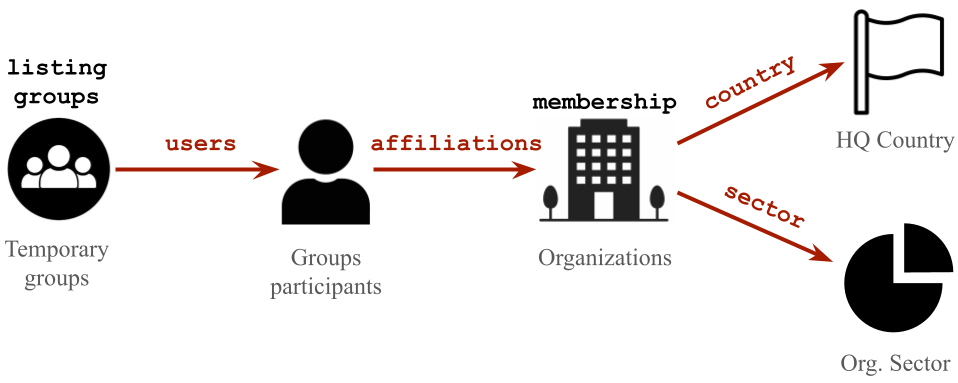
\includegraphics[width=0.9\columnwidth]{images/data-structure.png}
  \caption{Graph visualization of the data relations. Datasets with names in red establish connections between entities, while datasets with names in black provide entity properties used to list and filter the data.}
  \Description{Graph visualization of the data relations. The link between organizations and W3C groups is established by group participants, who are affiliated to organizations.}
  \label{fig:data-structure}
\end{figure}

At the time of data collection, there were 195 temporary groups in operation: 141 CGs, 43 WGs, 9 IGs, and 2 BGs. The \texttt{listing} data also includes references to task forces, which are teams charged with specific tasks and subordinated to other W3C groups. We opted not to include them in our analysis, as they are not independent. 

Group participants may figure in \texttt{affiliations} with up to two affiliations. In such cases, one is always "W3C invited expert". We opted to standardize the data by removing this affiliation when it is not the only one. This is because the invited expert affiliation is not an organization, but a status that allows individuals to participate in W3C groups without being affiliated to any organization. After this standardization, we were left with 147 invited experts with no other affiliation, which we classified as ``W3C Invited Experts''. Taking W3C and this pseudo affiliation into account, there were 303 organizations with at least one representative in W3C temporary groups at the time of data collection. About 21\% of the W3C member organizations were not participating in any group.

\section{Methodology}
\label{sec:methodology}

\subsection{Sector annotation with RAG}
\label{sec:lab}



\subsection{Topic modelling}


\section{Analysis}
\label{sec:analysis}

\subsection{Overall demographics}
\label{sec:demographics}

We first assessed the level of participation of member organizations in W3C groups by counting the number of representatives they have assigned to W3C temporary groups. This evaluation might hint us about organizations with the most capacity to influence the development of Web standards. Despite the W3C decision process being consensus-based where each organization has one vote, having representatives in multiple groups may improve the organization's ability to coordinate efforts across groups. Additionally, a larger number of representatives participating in a given group may sway the concrete consensus-building process in favor of that organization by creating the impression of a larger community support and by improving its arguing capabilities.

Fig. \ref{fig:reps-cum-fracs} presents the cumulative distribution of the number of representatives per organization for chartered (restricted to W3C members) and non-chartered groups (open to all organizations). The vertical dotted and dashed lines mark the number of organizations required to amass 50\% and 80\% of the representatives, respectively. We note that the concentration of group participants in a few organizations is larger in chartered than in non-chartered groups (Gini index of 0.68 versus 0.44). In chartered groups, half of all representatives are affiliated to the 20 largest among 397 organizations (5\%). By resampling 397 organizations from non-chartered groups, we concluded that the probability of reaching the chartered group Gini index by chance is 1.1\%, showing that the increased concentration seen in chartered groups requires a sociological explanation. One hypothesis would be that the W3C membership fee selects larger organizations or those more interested in W3C standards.

\begin{figure}[ht]
  \centering
  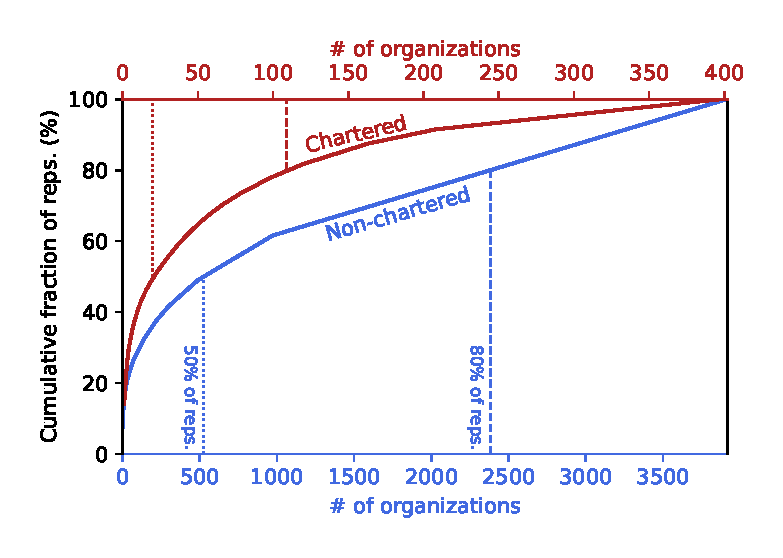
\includegraphics[width=1.0\columnwidth]{images/org-reps-cum-fracs.eps}
  \caption{Cumulative fraction of organization representatives participating in chartered (red) and non-chartered (blue) groups by number of organizations considered (ordered by decreasing number of representatives). For chartered groups, the number of organizations is referenced on the top horizontal scale, whereas for the non-chartered groups it is referenced on the bottom.}
  \Description{Bar plot showing the number of representatives per organization. Google is the largest organization in terms of representatives, having 693. It is followed by Microsoft, with 234, and W3C invited experts, Apple, Mozilla and Intel.}
  \label{fig:reps-cum-fracs}
\end{figure}

Fig. \ref{fig:reps-per-org} shows the number of W3C group participants that are affiliated to the top 20 largest organizations in terms of number of representatives, which all happen to be W3C members. Our hypothesis is that these organizations are the most influential in W3C. Google leads the list by a large amount (693 representatives), followed by Microsoft. Interestingly, apart from W3C invited experts, the top four organizations in plot are major browser vendors. 

\begin{figure}[ht]
  \centering
  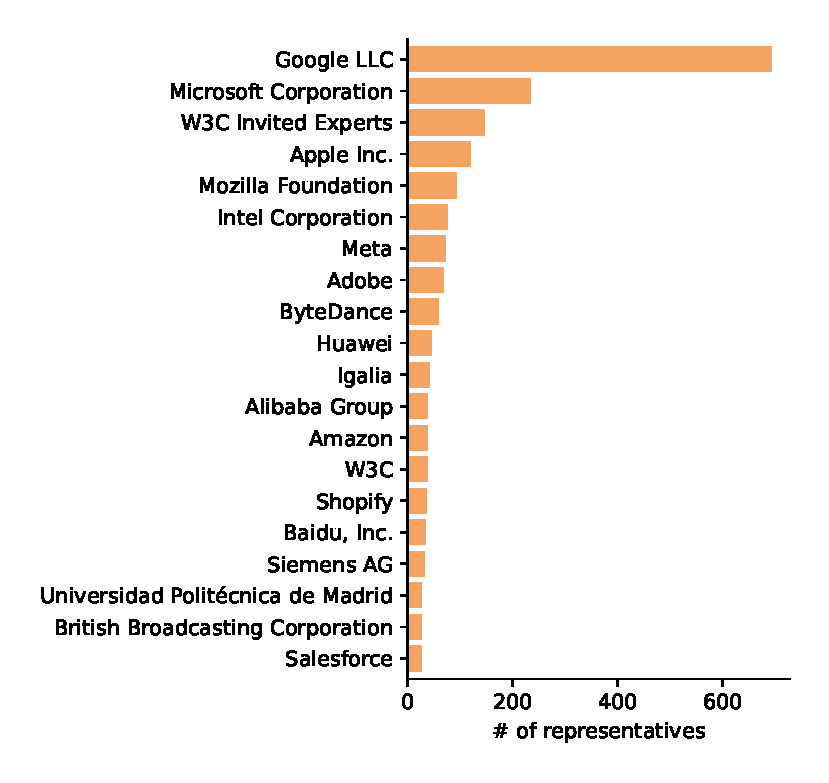
\includegraphics[width=1.0\columnwidth]{images/n-reps-per-org.eps}
  \caption{Number of representatives from the 20 largest organizations participating in W3C groups.}
  \Description{Bar plot shows a decreasing powerlaw-like trend. Google leads as the organization wih most representatives, with 3 times more than Microsoft, the second in the rank. It is followed by W3C Invited Experts, Apple, Mozilla, Intel, Meta, Adobe, ByteDance, Huawei, Igalia, Alibaba Group, Amazon, W3C, Shopify, Baidu, Siemens, Universidad Politécnica de Madrid, BBC, Salesforce. }
  \label{fig:reps-per-org}
\end{figure}

We aggregated the number of W3C member organization representatives by the country in which the organization's headquarters (HQ) is located. Fig. \ref{fig:reps-per-country} shows the results for the top 20 countries with most representatives, revealing the strong presence of organizations with HQ in the United States. It amassed 2,245 people, comprising 65.7\% of all W3C member representatives. This happened both because there are many member organizations in W3C from the United States and because some of these organizations have many representatives. Among the top 5 countries, USA, China, Japan, and UK also emerged as the owners' location of the world's most visited websites \cite{Xavier2024}. In contrast, Germany was well represented among W3C members but did not figure amidst the 116 most visited domains, whereas Russia was home of highly visited domains but had no members in W3C.\footnote{Note that Yandex participate in non-chartered groups, but not as a W3C member.} 

\begin{figure}[ht]
  \centering
  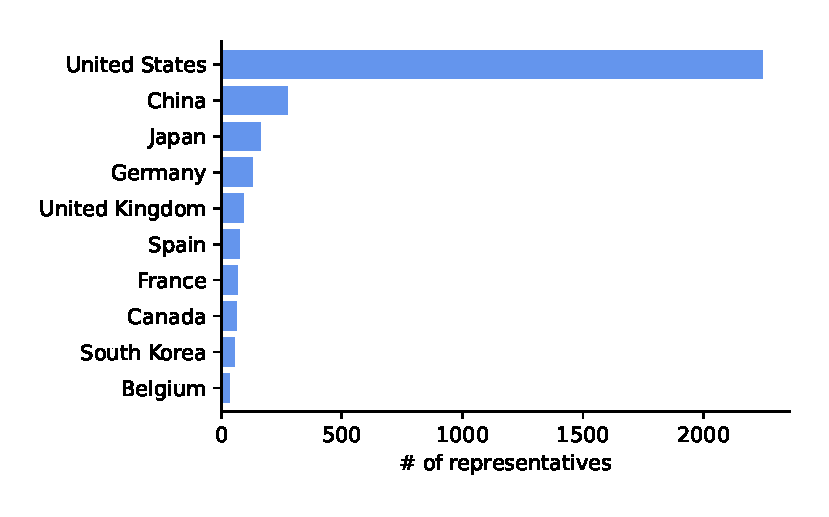
\includegraphics[width=1.0\columnwidth]{images/n-reps-per-country.eps}
  \caption{Number of W3C member representatives aggregated by member HQ country, for the top 10 countries with most representatives.}
  \Description{Bar plot showing a highly skewed powerlaw distribution, with United States leading with more than 8 times the next country with the most representatives: China. The latter is followed by Japan, Germany, UK, Spain, France, Canada, South Korea and Belgium.}
  \label{fig:reps-per-country}
\end{figure}

Fig. \ref{fig:reps-per-sector} presents the number of W3C member representatives aggregated by sector. Representatives from large enterprises are by far the most common participant. This is caused by the large number of W3C member organizations that are from this sector and also because such organizations are typically represented by a large team. Conversely, the average Small/Medium enterprise have the smallest number of representatives of all sectors.

\begin{figure}[ht]
  \centering
  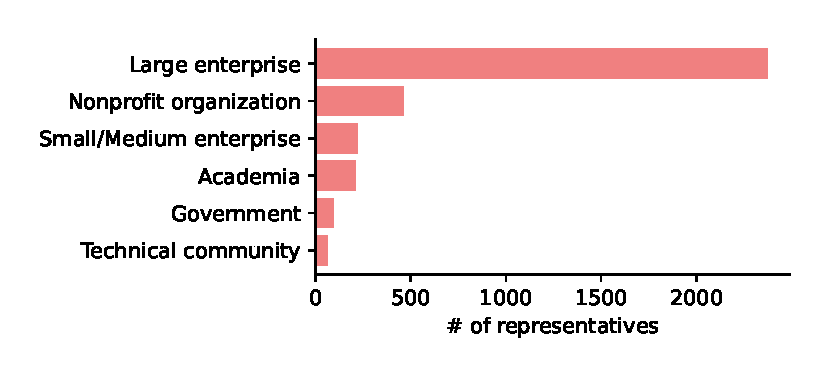
\includegraphics[width=1.0\columnwidth]{images/n-reps-per-sector.eps}
  \caption{Number of W3C member representatives aggregated by member sector.}
  \Description{Large enterprises is the sector with the most representatives, with 5 times more than Nonprofit organizations, in second place. This is followed by Small/Medium enterprises, Academia, Government and Technical Community.}
  \label{fig:reps-per-sector}
\end{figure}

\subsection{Topic modelling}



\section{Summary and conclusions}
\label{sec:conclusions}

\bibliographystyle{ACM-Reference-Format}
%\bibliographystyle{natbib}
\bibliography{main}

\balance

\appendix

\section{Annotated data}
\label{sec:annotations}

\end{document} 
